\section{Инструкции по работе с 1С Розница}

\subsection{Создание документа "Приказ на пересчет товаров" по избранной номенклатуре}

\begin{itemize}
	\item Для того что бы можно было выполнять "частичную" инвентаризацию по группам номенклатуры, необходимо заполнить справочник "Правила отбора товаров".   Это операция выполняется однократно. 
\end{itemize}	
\begin{enumerate}	
	\item Справочник "Правила отбора товаров" находится в разделе "Склад" Рис.~\ref{ris:0_2.jpg}
	\item Необходимо открыть справочник Рис.~\ref{ris:0_2.jpg}
	\begin{figure}[H]
		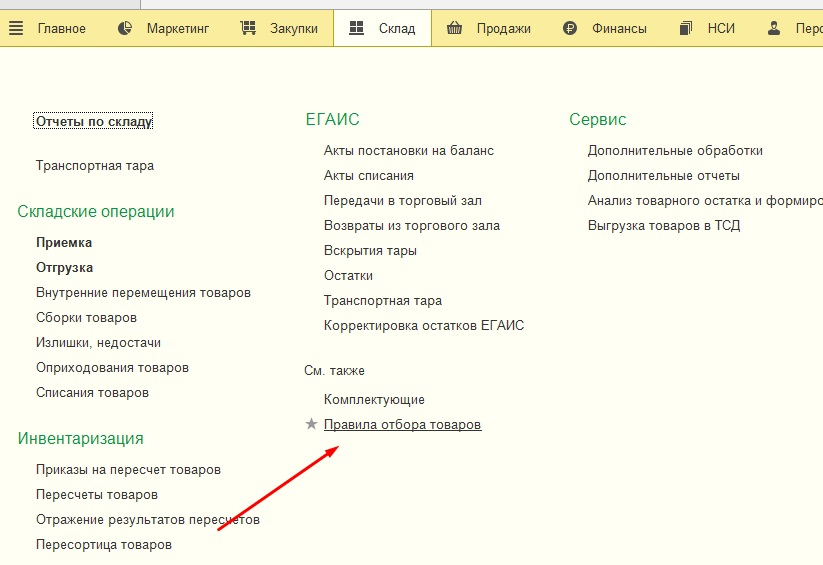
\includegraphics[width=0.45\textwidth]{0_2.jpg}
		\caption{Расположение справочника Правила отбора товаров .}
		\label{ris:0_2.jpg}
	\end{figure}
	\begin{figure}[H]
		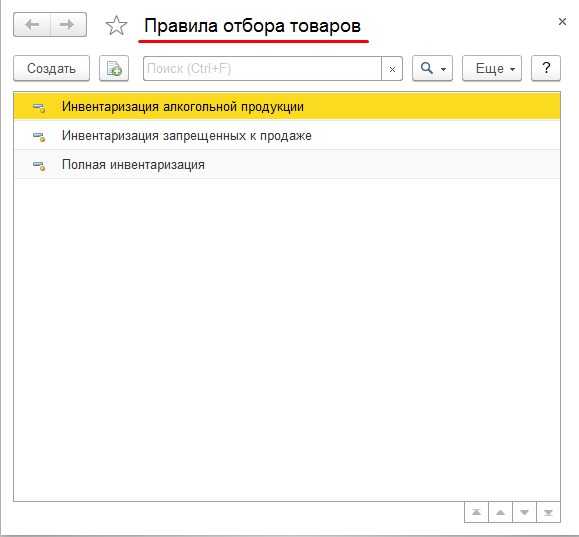
\includegraphics[width=0.4\textwidth]{0_3.jpg}
		\caption{Справочник Правила отбора товаров .}
		\label{ris:0_3.jpg}
	\end{figure}	
	\item Далее выбрать создание нового элемента. Рис.~\ref{ris:0_4.jpg} Используя кнопку "Создать" или клавишу "Insert"  на клавиатуре.	
	\begin{figure}[H]
		\center{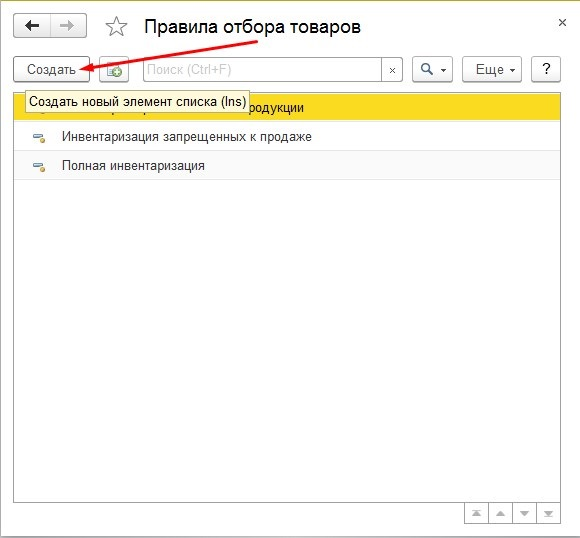
\includegraphics[width=.4\linewidth,keepaspectratio]{0_4.jpg}}
		\caption{Справочник Правила отбора товаров создать .}
		\label{ris:0_4.jpg}
	\end{figure}
	\item Заполнить наименование нового отбора. Рис.~\ref{ris:0_5.jpg}	
	\begin{figure}[H]
		\center{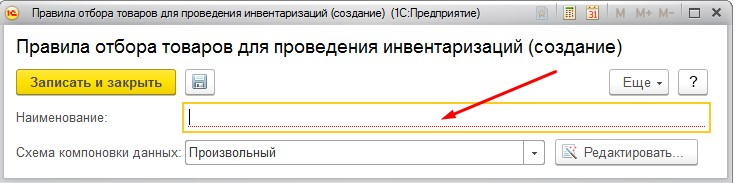
\includegraphics[width=.4\linewidth,keepaspectratio]{0_5.jpg}}
		\caption{Справочник Правила отбора товаров задать наименование.}
		\label{ris:0_5.jpg}
	\end{figure}
	\item Открыть новое правило на редактирование. Рис.~\ref{ris:0_6.jpg}	
	\begin{figure}[H]
		\center{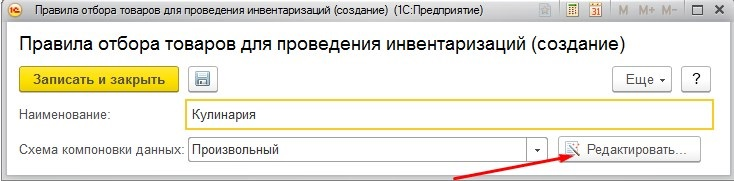
\includegraphics[width=.4\linewidth,keepaspectratio]{0_6.jpg}}
		\caption{Справочник Правила отбора редактирование отбора.}
		\label{ris:0_6.jpg}
	\end{figure}
	\item После нажатия на кнопку "Редактировать" откроется настройка схемы для формирования нужного отбоора. В списке доступных полей слева нужно выбрать необходимое поле. В данном случае это будет "Номенклатура. Рис.~\ref{ris:0_7.jpg} Двойным кликом левой кнопки мыши или с помощью кнопки "Выбрать, переносим поле "Номенклатура в правую часть.  Рис.~\ref{ris:0_8.jpg} Затем в колонке "Вид сравнения" нужно выбрать требуемый вид сравнения. Если выбрать "В группе из списка", тогда в отбор для инвентаризации попадет та номенклатура, которая входит в группу указанную в поле "Значение". Если выбрать "Не в группе из списка", то соответственно в отбор для инвентаризации попадет вся номенклатура, которая не входит в выбранную группу. 
	Аналогично можно воспользоваться другими видами сравнения.
	
	\begin{figure}[H]
		\center{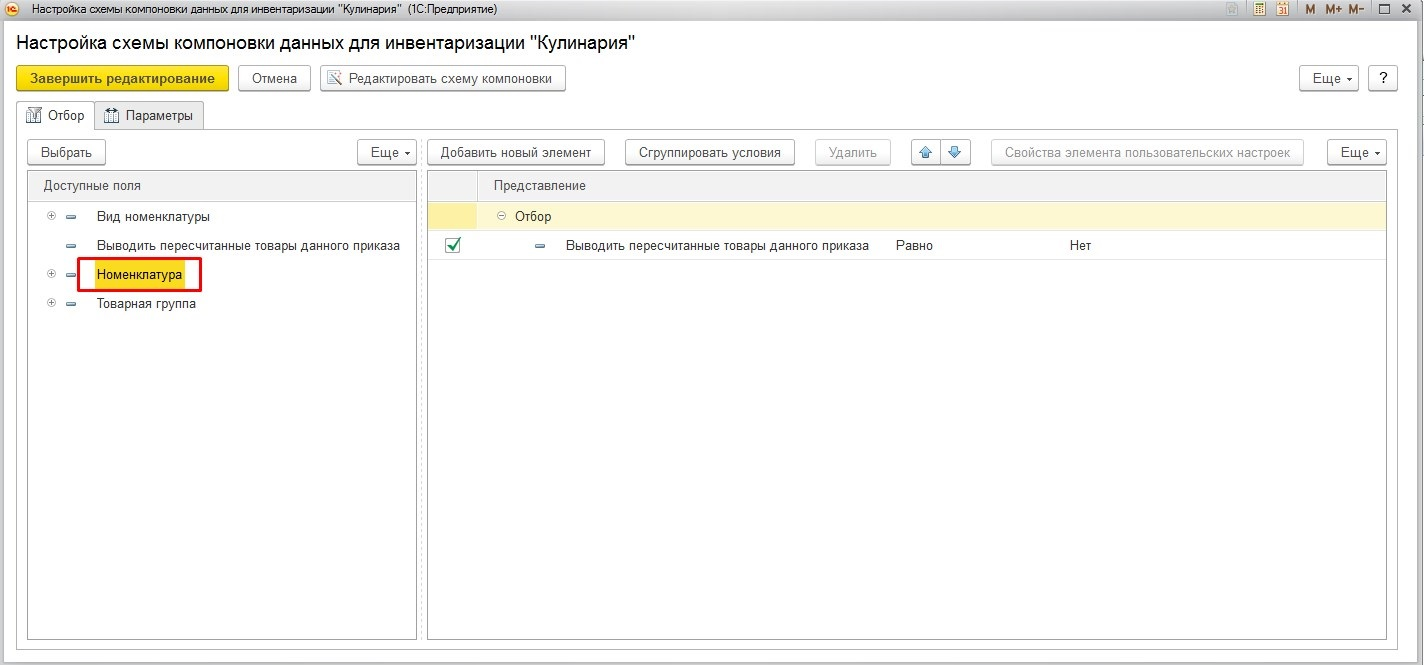
\includegraphics[width=.4\linewidth,keepaspectratio]{0_7.jpg}}
		\caption{Выбор из доступных полей.}
		\label{ris:0_7.jpg}
	\end{figure}
	\begin{figure}[H]
		\center{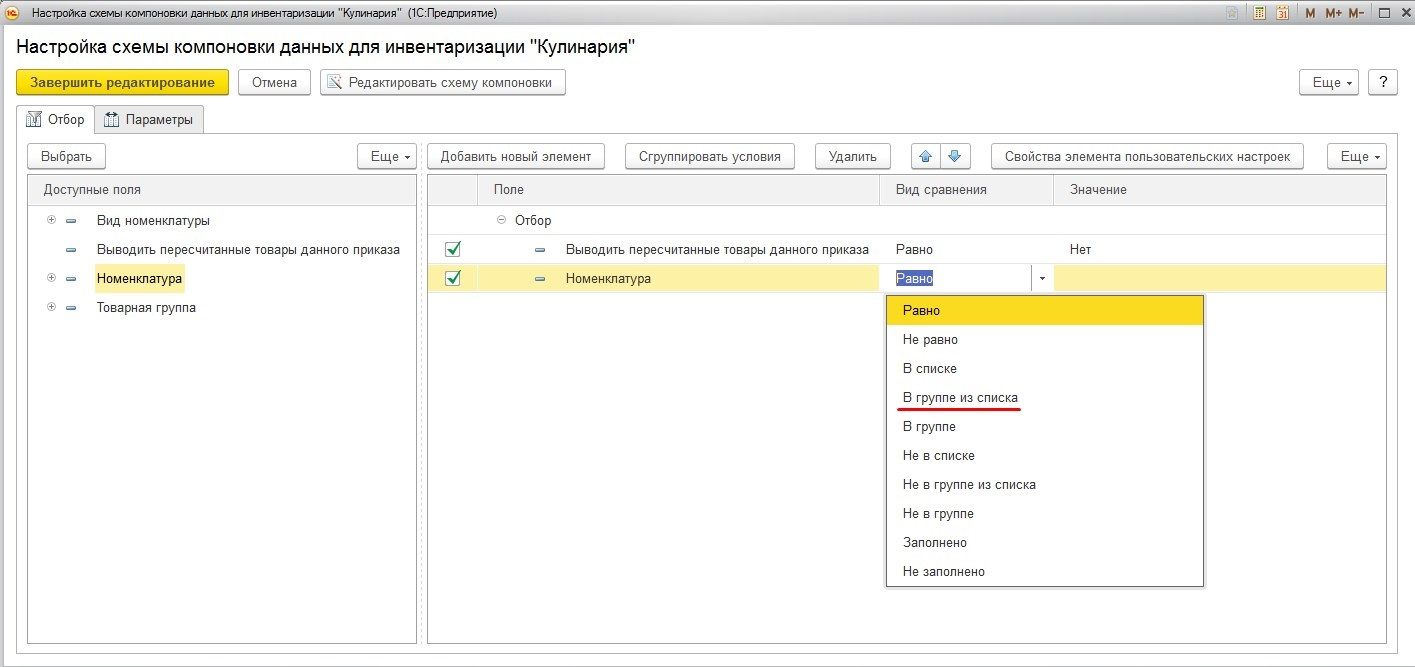
\includegraphics[width=.4\linewidth,keepaspectratio]{0_8.jpg}}
		\caption{Выбор вида сравнения.}
		\label{ris:0_8.jpg}
	\end{figure}
	\item В открывшееся окне "Список значений" Рис.~\ref{ris:0_9.jpg}, используя кнопку "Добавить" добавляем нужные нам группы номенклатуры. Рис.~\ref{ris:0_10.jpg}
	\begin{figure}[H]
		\center{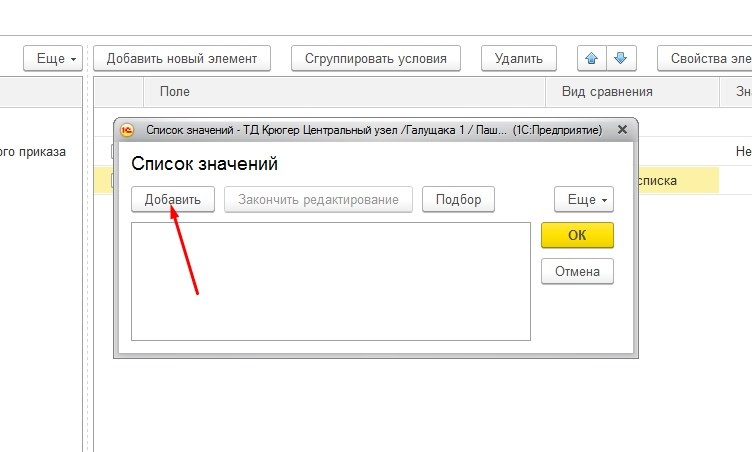
\includegraphics[width=.4\linewidth,keepaspectratio]{0_9.jpg}}
		\caption{Выбор из доступных полей.}
		\label{ris:0_9.jpg}
	\end{figure}
	\begin{figure}[H]
		\center{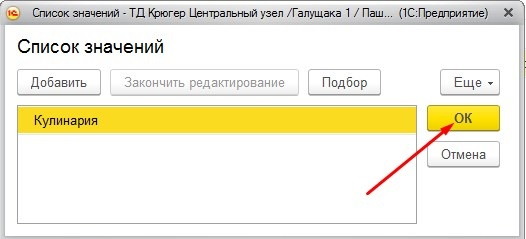
\includegraphics[width=.4\linewidth,keepaspectratio]{0_10.jpg}}
		\caption{Выбор вида сравнения.}
		\label{ris:0_10.jpg}
	\end{figure}
		\item Нажимаем кнопку "Ок" и закрываем список. Закрываем настройки схемы Рис.~\ref{ris:0_11.jpg}, Закрываем настройку правил. Рис.~\ref{ris:0_12.jpg}
		Теперь у нас появилось новой правило отбора и его можно использовать в документе  "Приказ на пересчет товаров". Возможно создавать практически любое количество правил для отбора номенклатуры и использовать их  впоследствии в своей работе. Рис.~\ref{ris:0_13.jpg}
	\begin{figure}[H]
		\center{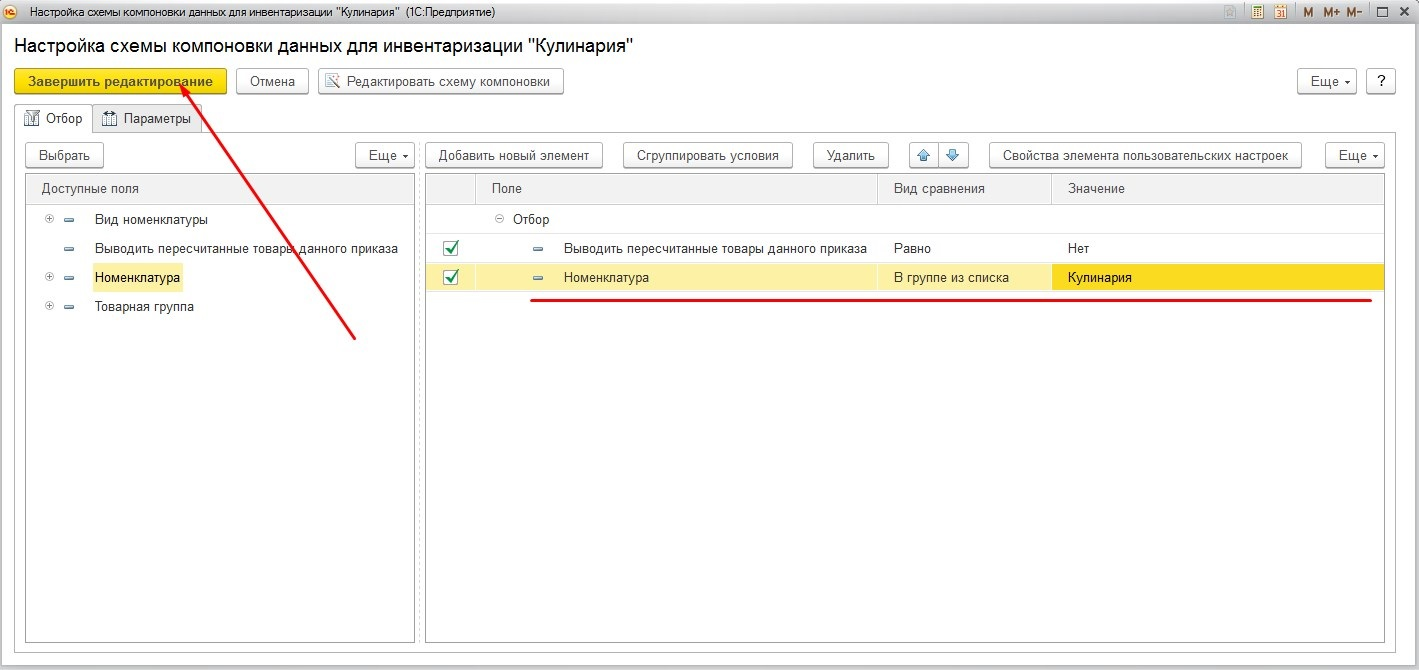
\includegraphics[width=.4\linewidth,keepaspectratio]{0_11.jpg}}
		\caption{Закрыть настройку схемы.}
		\label{ris:0_11.jpg}
	\end{figure}
	\begin{figure}[H]
		\center{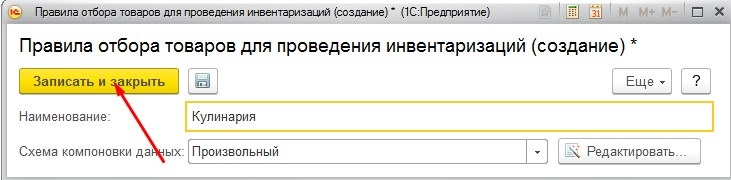
\includegraphics[width=.4\linewidth,keepaspectratio]{0_12.jpg}}
		\caption{Закрыть настройку правил.}
		\label{ris:0_12.jpg}
	\end{figure}

	\begin{figure}[H]
		\center{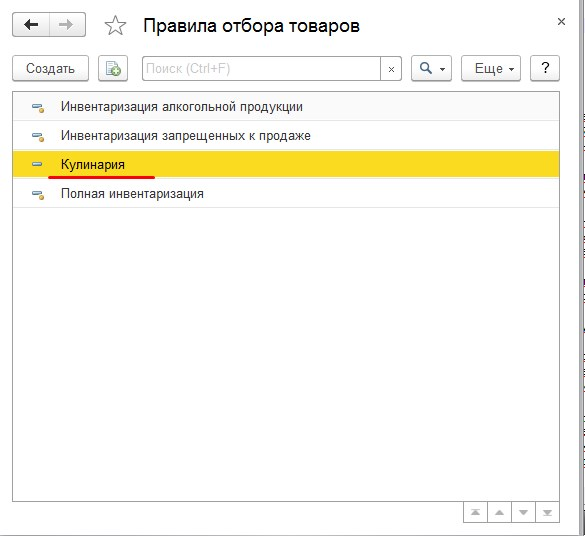
\includegraphics[width=.4\linewidth,keepaspectratio]{0_13.jpg}}
		\caption{Список правил.}
		\label{ris:0_13.jpg}
	\end{figure}
	\item Теперь переходим к документу "Приказ на пересчет товаров" находящемуся в разделе "Склад" Рис.~\ref{ris:0_1.jpg}
	\begin{figure}[h!]
		\center{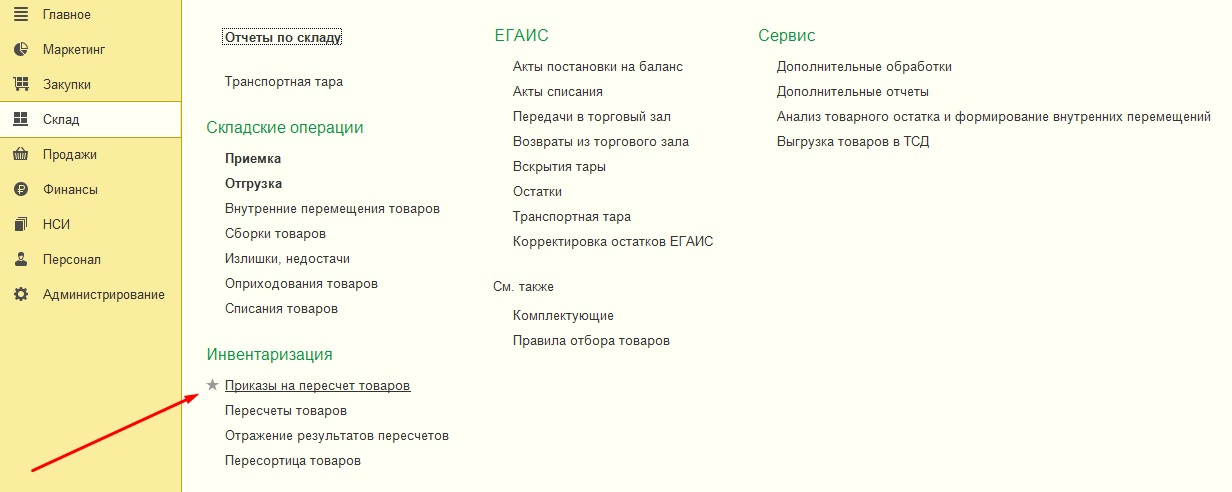
\includegraphics[width=.9\linewidth,keepaspectratio]{0_1.jpg}}
		\caption{Расположение документа.}
		\label{ris:0_1.jpg}
	\end{figure}
	\item "Кликаем" мышкой и открываем список документов "Приказ на пересчет товаров", создаем новый документ использую клавишу "Insert" на клавиатуре, либо кнопку "Создать" в списке.
\begin{figure}[H]
	\center{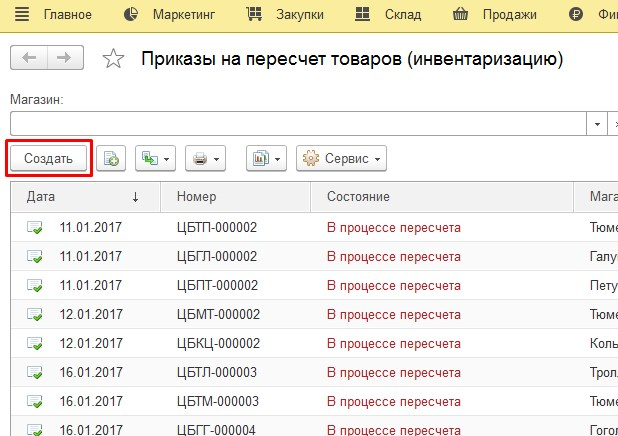
\includegraphics[width=.48\linewidth,keepaspectratio]{0_17.jpg}}
	\caption{Создание документа.}
	\label{ris:0_17.jpg}
\end{figure}
	\item В новом документе необходимо заполнить все реквизиты в шапке. 
	Реквизит "Отбор" заполняем нужным значением. 
	\begin{figure}[H]
		\center{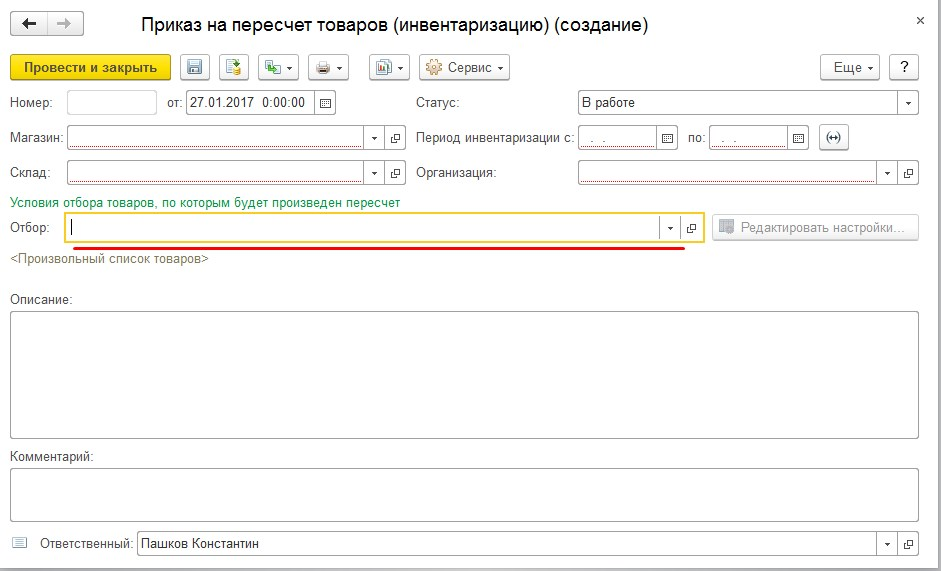
\includegraphics[width=.4\linewidth,keepaspectratio]{0_14.jpg}}
		\caption{Реквизит "Отбор".}
		\label{ris:0_14.jpg}
	\end{figure}
	\begin{figure}[H]
		\center{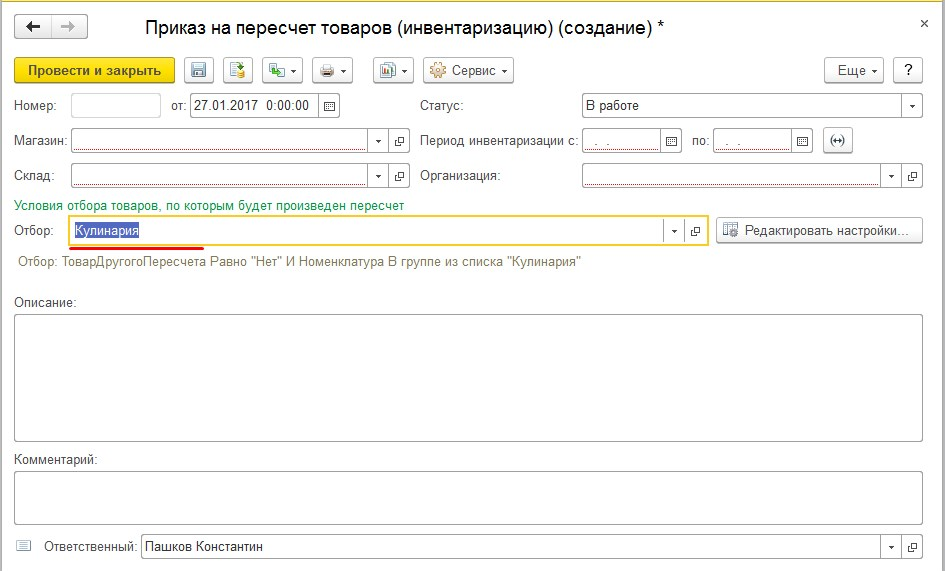
\includegraphics[width=.4\linewidth,keepaspectratio]{0_16.jpg}}
		\caption{Заполненный реквизит "Отбор".}
		\label{ris:0_16.jpg}
	\end{figure}	
	\item Теперь в документы созданные на основании данного, при заполнении попадут только те позиции номенклатуры, которые были указаны в выбранном отборе.
	\end{enumerate}

